\documentclass[12pt,a4paper]{article}

\usepackage[utf8]{inputenc}
\usepackage{graphicx}
\usepackage[spanish]{babel}
\usepackage{float}				%Para poner las imagenes exactamente donde se me cante las pelotas en caso de quererlo, poniendole [H]
\usepackage{amsmath}
\usepackage{epstopdf}
\usepackage{geometry}
\usepackage{hieroglf}
\usepackage{subcaption}
\usepackage[justification=centering]{caption}
\usepackage[colorlinks=true, allcolors=blue]{hyperref}
\geometry{
a4paper,
left=20mm,
right=20mm,
top=25mm,
bottom = 20mm
}
\usepackage{float}
\usepackage{units}
\marginparwidth=2cm
\usepackage[colorinlistoftodos]{todonotes}

% \usepackage{hyperref}   %Esto es para ir a los links

\title{\mathbf{Mecánica de Medios Continuos \\Práctica 4 \\ Tensión}}

\author{Universidad de Cuenca}
\begin{document}
\maketitle
\begin{enumerate}
    \item 
    La compuerta A-B de la figura puede rotar alrededor del eje A. Tiene forma de un cuarto de cilindro de radio R y longitud L
    en la dirección perpendicular al plano de la hoja.
    \begin{enumerate}
        \item Obtenga la expresión del vector de fuerza por unidad de volumen $mathbf{b}$
        \item  Despreciando la presión atmosférica y considerando que el nivel del agua
        llega hasta la altura B, calcular la fuerza que se debe aplicar en el punto B para mantener la compuerta en equilibrio.
    \end{enumerate}
    \begin{figure}[h]
        \centering
        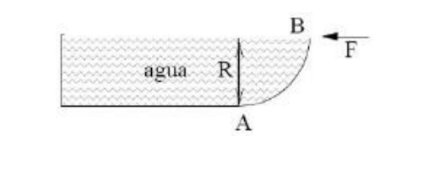
\includegraphics[width=0.6\textwidth]{tp4-1.png}

    \end{figure}
    \item Considere un recipiente cilíndrico de radio R y altura 2H
    que rota con frequencia angular $\omega$
    alrededor de su eje. Dentro del recipiente hay un líquido incompresible,
    cuyo volumen es la mitad del volumen del recipiente, que rota uniformemente con la
    misma frequencia angular.
    \begin{enumerate}
        \item Determinar la forma funcional de la superficie libre del líquido.
        \item Determinar el valor de la frecuencia $\omega_0$
        a partir de la cual la superficie libre
        comienza a tocar el fondo del recipiente.
        \item Calcular la distribución de presión sobre las paredes y en el fondo del recipiente
        en el caso en que el fluido se encuentre en reposo, y cuando rota.
    \end{enumerate}
    \item Los vectores de tracción $\mathbf{t^{(1)}, t^{(2)}}$ y $\mathbf{t^{(3)}}$ en un punto de un medio continuo son:   
    \begin{align}
        \mathbf{t^{(1)}} &= (1,2,0) \\
        \mathbf{t^{(2)}} &= (2,1,0) \\
        \mathbf{t^{(3)}} &= (0,0,1)
    \end{align} 
    Encuentre el tensor de Cauchy.
    \item Suponga que el tensor de Cauchy de un medio continuo en un punto $\mathbf{x}$ está dado por.
    \begin{equation}
        [\sigma]=\begin{pmatrix}
            5 & 3 & -3\\
            3 & 0 & 2\\
            -3 & 2 & 0
            \end{pmatrix}
    \end{equation}
    Y considere una superficie $\Gamma$ con vector normal $\mathbf{n}=(0,1/\sqrt{2},1/\sqrt{2})$.
    \begin{enumerate}
        \item Encuentre el vector de tracción en la superficie $\Gamma$ en el punto $\mathbf{x}$.
        \item Encuentre las deformaciones principales en $\mathbf{x}$ y sus direcciones.
    \end{enumerate}
\end{enumerate}
\end{document}